\chapter{Revue de la littérature}
Nous présentons dans ce chapitre un état de l’art des méthodes d'ingénierie de ligne de produits. Dans un premier temps, nous parcourrons les concepts de l'ingénierie de ligne de produits acceptés des chercheurs du domaine. Ensuite nous présentons quelques plateformes existantes de l'ingénierie de ligne de produits. 

\section{Ingénierie de lignes de produits}
En réponse à la difficulté de produire des logiciels de qualité à moindre coût et en respectant les délais, les industries et les universités se sont penchées, autour des années 2000, vers une nouvelle idéologie consistant à produire des familles de logiciels plutôt que des logiciels indépendants: c'est l'ingénierie de ligne de produits logiciels. L’idée derrière les LPL est de maximiser la production de logiciels présentant des similarités, issus d’une même famille de produits, par la réutilisation systématique d’une même base de code et par la définition de variantes \cite{Urli2015}. 

Clements et al. \cite{Clements2002} définissent une famille de logiciels ou ligne de produits logiciels (LPL) comme \glsdesc{LPL_def}. Cette définition fait ressortir le fait que les logiciels d'une famille sont développés à partir du même ensemble d’artefacts logiciels et repondent chacun à un besoin spécifique bien que provenant d'une base commune de code. L’ingénierie de ligne de produits ne vise donc pas à produire des logiciels pour satisfaire un besoin isolé comme traditionnellement, elle vise plutôt la satisfaction d'une large gamme de besoins dans un secteur d'activité ou domaine donné. Chaque logiciel de la famille répondant à un besoin particulier de ce domaine et ayant des points communs avec les autres logiciels de sa famille et ses propres spécificités qui le différencient des autres, communément nommées variantes. Elle tire avantage de la réutilisation de code et la personnalisation de masse. Le domaine est d'abord minutieusement étudié, une fois la ligne de produit construite, le développement d'un logiciel membre se fait par configuration de la plate-forme support et la réutilisation de composants pour répondre aux besoins spécifiques.

Le processus de développement des lignes de produits se fait en deux étapes, l'ingénierie du domaine et l'ingénierie de l'application. Le produit final étant une architecture qui servira de socle au développement des produits du domaine et des composants réutilisables qui seront exploités lors de la production des logiciels de la famille. La figure \ref{fig:framework_ILP} ci-dessous présente le Framework de l'ingénierie de ligne de produits.

\begin{figure}[h!]
  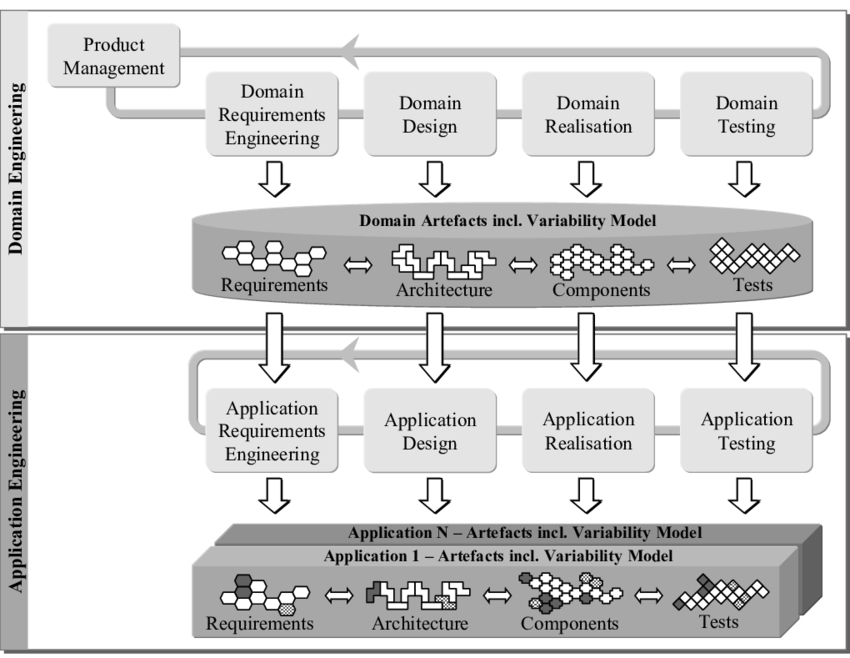
\includegraphics[scale=0.9999, width=150mm]{images/SPLE_Framework.png}
  \caption{framework de l'ingénierie de ligne de produits}
  \label{fig:framework_ILP}
\end{figure}

\subsection{Ingénierie de domaine}
Le développement d'une ligne de produits logiciels nécessite une bonne compréhension du domaine concerné et une fluide expression de la variabilité, qui est l'ensemble des propriétés qui diffèrent d'une application à une autre. Un domaine peut être vu comme \glsdesc{domaine} \cite{Klaus2005}. L'ingénierie de domaine est alors \glsdesc{ingenierie_de_domaine} \cite{Klaus2005}. Elle se réalise en trois phases:
\begin{itemize}
	\item \textbf{l'analyse du domaine} qui est l'activité qui décrit et représente formellement les concepts de base du domaine ainsi que la variabilité. Avant de faire une analyse du domaine, il faut au préalable définir les frontières du domaine à analyser. Elle vise à réaliser un modèle du domaine qui spécifie formellement les informations de celui-ci. Une bonne analyse de domaine se mène en plusieurs activités: la définirion du dictionnaire des termes du domaine, la documentation des hypothèses du domaine, l'identification des acteurs du domaine, l'identification des problèmes du domaine, l'identification des artéfacts existants et l'identification de la similarité et de la variabilité.
	\item \textbf{la spécification de l’infrastructure}, Elle prend en entrée le modèle produit à l'étape précédente et décrit l’organisation des artefacts réutilisables (spécifications, diagrammes, code etc.),
	\item \textbf{l’implémentation de l'infrastructure} qui comprend l’implémentation des artefacts définis à l'étape précédente
\end{itemize}  
\subsection{Ingénierie de l’application}
Elle permet de developper les nouvelles applications du domaine à partir de la plate-forme et des composants réutilisables créés aucours de l'ingénierie de domaine. La réalisation du produit durant l’ingénierie de l’application est généralement automatisée à partir des choix effectués au sein de la représentation abstraite définie lors de l’ingénierie du domaine \cite{Awais2011}. La production des produits logiciels se fait par la configuration de la plateforme et la réalisation du produit qui est souvent automatisée. Cette derniere activité fait intervenir des techniques avancées de l'ingénierie logicielle telles que l’ingénierie dirigée par les modèles et la programmation générative \cite{Urli2015}. L'ingénierie de l'application suit un cycle de vie <<classique>> où chaque étape est facilitée par les artéfacts de l'ingénierie de domaine.
\begin{itemize}
	\item \textbf{Analyse des besoins} La définition des besoins.
	\item \textbf{Conception de l'application} La spécification de la solution permettant de satisfaire ces
besoins.
	\item \textbf{Implémentation} L’implémentation de cette solution.
	\item \textbf{Tests et validation} La phase de test de la solution et son évaluation par
rapport aux besoins initiaux.
\end{itemize}
\subsection{Introduction à la variabilité}
Les applications d'une LPL ont certes beaucoup de points communs mais aussi des différences que l'on exprime par la notion de variabilité. La variabilité peut être définie comme \glsdesc{variabilite} \cite{Hugo2013}. Pour maîtriser cette variabilité, il faut distinguer "le sujet de la variabilité" (ce qui varie), de "l'objet de la variabilité" (comment cela varie) et du "point de variiation" (comment la variabilité se réalise au sein de la ligne). Pol et al. \cite{Klaus2005} résument cela en trois questions:

\begin{itemize}
	\item  Qu'est ce qui varie ?
	\item Pourquoi est-ce-que cela varie ?
	\item Comment cela varie-t-il ?
\end{itemize}
Les assertions suivantes font ressortir des propriétés qui varient: 

\begin{itemize}
	\item  Une voiture peut avoir un toit fixe ou ouvrant.
	\item Une personne a des enfants qui peuvent être des garçons ou des filles.
	\item Un ordinateur peut être équipé d’une deuxième batterie ou d’un lecteur de DVD.
\end{itemize}
Il est donc question d'intégrer la variabilité dans les artefacts réutilisables dès l'analyse du domaine et dans toutes les autres phases (elle est intégrée dans le modèle du domaine, les spécifications, l'architecture, les composants, les scénarios de test etc. \cite{Magnus2003}). Le but étant d’accroître la flexibilité de la plate-forme et des composants. Lorsque cela est bien fait, la dérivation d'un produit membre se fait essentiellement par la sélection des bons artefacts et la génération du code source.
\subsection{Modélisation de la variabilité}
Dans la littérature, plusieurs approches ont été proposées pour modéliser la variabilité. Une des plus acceptées est la méthode \textbf{FODA} \glsdesc{FODA} basée sur les \textsl{features} proposée par Kang et al. en 1990. Un feature ou caractéristique métier est \glsdesc{feature} \cite{Kyo1990}. La méthode FODA distingue trois types de caractéristiques métiers:

\begin{itemize}
	\item  Les caractéristiques obligatoires, qui sont communes à tous les produits de la ligne.
	\item Les caractéristiques optionnelles, qui sont facultatives.
	\item Les caractéristiques alternatives. C'est un petit ensemble dont on ne peut choisir qu'un élément à un moment donné.
\end{itemize}

\section{Les plateformes de Lignes de produits}
\subsection{FAMA}
FAMA(FeAture Model Analyser) \cite{Benavodes2007} est un Framework d’analyse automatique des Feature Models dans les LPL. En effet, la gestion des grands Features Models avait déjà été décrite dans la littérature comme une tâche difficile et sujette à des erreurs. Ces Features Models contiennent des informations très utiles comme par exemple le nombre de produits potentiel modélisés, les features du noyau de la plateforme et les features variants de la ligne de produit. FAMA se propose alors d'analyser automatiquement les features models et d'en extraire les informations utiles et détecter des éventuelles erreurs. Le modèle théorique de FAMA est basé sur les Features Models étendus avec des cardinalités sur lesquels on applique la programmation par contraintes. Un exemple de CSP(Constraint Satisfaction Problem) est donné par l'illustration suivante.
\begin{figure}[h!]
  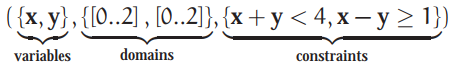
\includegraphics[scale=0.9999, width=150mm]{images/exemple_constraint_satisfaction_problem.PNG}
  \caption{Exemple de problème satisfaisant une contrainte \cite{Benavodes2007}}
  \label{fig:FORM_Process}
\end{figure}

L'analyse d'un Feature Model se fait en deux étapes: il est d'abord traduit en une représentation logique puis des solveurs procèdent à l'extraction des informations. Un prototype nommé FAMA-EP a été développé en tant que plug-in Eclipse. Il offre deux principales fonctionnalités: la création et la modification visuelle de modèles et l'analyse automatique de ces modèles. Une fois que l'utilisateur crée ou importe un Feature Model, l'analyse peut commencer. FAMA-EP intègre plusieurs solveurs pour l'analyse pour plus d'efficacité. Il permet entre autre de déterminer si un feature model est non vide (s'il peut produire au moins un produit), trouver le nombre total de produits, lister tous les produits possibles du Feature Model, calculer l'ensemble de features communs. 
L'architecture de ce plug-in se constitue d'un éditeur visuel et d'un moteur d'analyse qui se charge de trouver le meilleur solveurs pour effectuer l'analyse demandée sur le Feature Model. Nous notons que FAMA est éfficace pour l'analyse des Features Models puisqu'il utilise plusieurs solveurs cependant il ne couvre pas toutes les étapes de l'ingénierie de ligne de produit.
 
\subsection{PURE::VARIANTS}
PURE::VARIANTS \cite{PureVariants} est une plateforme professionnelle, livrée comme plug-in Eclipse ou standalone application pour supporter le développement et le déploiement des lignes de produits logiciels. La ligne de produits logiciels est ici décrite en trois parties principales; Feature Models, Family Models et Variant Description Model. \textbf{Le Feature Model} décrit les produits de la ligne en terme de features qui sont communs à ces produits et de features qui varient d'un produit à un autre ainsi que les relations entre ces features; un feature étant une propriété d'un produit qui sera visible par l'utilisateur du produit. \textbf{Le Family Model} quant à lui décrit comment les produits de la ligne seront assemblés ou générés à partir des composants existants; chaque composant représente un ou plusieurs éléments fonctionnels des produits de la ligne (classes, objets, variables etc.). Chaque élément du Family Model a des contraintes qui spécifient s'il doit être inclus, par défaut tout élément dont le parent est inclus est également inclus. \textbf{Le Variant Description Model} (VDM) décrit l'ensemble des features d'un produit de la ligne. C'est dans ce modèle que l'on indique les features à choisir parmi ceux du Feature Model pour un produit spécifique à générer. PURE::VARIANTS offre un editeur pour spécifier et valider les features pour la configuration d'un produit (\textit{VDM editor}). Plusieurs versions de PURE::VARIANTS sont en vente en ligne parmi lesquelles PURE::VARIANTS for AUTOSAR pour la création et la maintenance des modèles réutilisables AUTOSAR, PURE::VARAINTS for IBM Rationnal Doors pour la gestion de la varaibilité dans les besoins fonctionnels des applications, PURE::VARAINTS for Enterprise architect pour la création et la maintenance des modèles UML et SysML.
 
\subsection{FeatureIDE}
FeatureIDE \cite{hum2012} est un framework gratuit basé sur Eclipse qui supporte les étapes du développement de logiciel basé sur les features. Il supporte plusieurs techniques d'implémentation des logiciels à partir des features telles que la programmation orientée feature, la programmation par aspects, la programmation orientée Delta et  les préprocesseurs. Le but principal de cet outil est de couvrir le cycle complet de développement et d'incorporer les outils dans des environnements de développement intégré (EDI). Son architecture facilite le développement d'outils supports pour les langages existants et les nouveaux langages pour les lignes de produits. FeatureIDE est beaucoup plus un outil pour la recherche et l'enseignement. Il est utilisé à Austin (au Texas), Magdebourg (en Allemagne), Marbourg (en Allemagne), Santa Cruz (en Californie), Turin (en Italie). Cet outils pourvoit un éditeur graphique de features Models qui permet de construire des features models en ajoutant et en enlevant des features. Cet éditeur permet de déplacer un feature (avec ses sous-features) sur un nouveau feature parent. FeatureIDE en lui même se concentre sur l'analyse du domaine; pour couvrir le cycle complet de l'ingénierie de ligne de produit, des extensions doivent être ajoutée au framework pour supporter l'implémentation du domaine et la génération de logiciel. Plusieurs extensions implémentant diverses approches sont disponibles. AHEAD, FeatureHouse, FeatureCpp, DeltaJ, AspectJ, Munge en sont quelques unes.  
       
\subsection{SPLOT}
SPLOT(Software Product Line Online Tool) \cite{Marcilio2009} est un système web développé en java qui utilise un générateur de template HTML pour créer des environnements hautement interactifs avec des interfaces utilisateurs de raisonnement et de configuration basées sur Ajax(Asynchronious Javascript And XML). Puisqu'il est basé sur internet, il facilite grandement le partage de connaissance notamment à travers le dépôt de features models et ne nécessite pas de téléchargement de mises à jour . Il offre deux principaux services: le raisonnement automatisé et la configuration du produit. Le raisonnement est axé sur l’automatisation du calcul statistique (profondeur de l'arbre de features, nombre de features etc.) et le débogage critique (cohérence des features models, détection des features morts etc.). Disponible en ligne à l'adresse \textsl{http://splot-research.org}, SPLOT a un riche dépôt de features models contenant près de 20 modèles réels précedement publiés dans la litterature et plusieurs modèles générés. L'éditeur graphique de feature de SPLOT permet de modifier un des modèles existants ou d'en créer un nouveau. Il permet d'ajouter un nouveau feature obligatoire, optionnel ou un groupe de features alternatifs. L'ajout des règles entre features dans SPLOT se fait en ajoutant des règles sous la forme de conjonction de littéraux dans laquelle les littéraux sont des features ou leur négation. A titre d'exemple pour signifier que l'inclusion d'un feature A oblige l'inclusion d'un feature B, la règle s'écrit comme suit: 
\lnot$FeatureA  \lor$ FeatureB. Pour rendre ette proposition vraie, le Feature A et le Feature B doivent être sélectionnés mais elle est également vraie quand le Feature B est choisi et pas Feature A. 

\subsection{Points de comparaison entre ces outils}
Nous dressons ci-dessus un tableau comparatif des outils de ligne de produits précédemment décrits. Les critères arrétés pour cette analyse sont les suivants:
 
 \begin{itemize}
	 \item  La portée: qui définit si le logiciel est open source ou à but commercial
	 \item  Le langage utilisé pour développer l'outil
	 \item  L’existence d'un éditeur de features intégré dans l'outil
	 \item  l'existance d'une description formelle de l'éditeur visuel qui permet de bien comprendre l'architecture interne de l'éditeur et l'étendre au besoin.
 \end{itemize}

\begin{table}[b]
\begin{tabular}{|l|c|c|c|r|}
  \hline
  \textbf{Outils} & \textbf{Portée} & \textbf{Langage} & \textbf{Editeur intégré} & \textbf{Description formelle} \\
	\hline
  \textsl{FAMA} & open source & Java & oui & non \\
  \hline
  \textsl{PURE::VARIANTS} & commerciale & Java & oui & non \\
	\hline
  \textsl{FeatureIDE} & open source & Java & oui & non \\
	\hline
  \textsl{SPLOT} & open source & Java & oui & non \\
	\hline
  \textbf{REAL} & \textbf{open source} & \textbf{Java} & \textbf{oui} & \textbf{oui} \\
  \hline
\end{tabular}
\caption{Tableau comparatifs des outils de LPL\label{time}} 
\end{table}

Nous faisons la remarque selon laquelle le langage Java et la plateforme Eclipse sont très utilisés pour le développement d'éditeurs de features mais ces derniers manquent le plus souvent de description formelle. Pourtant une bonne description formelle des éditeurs faciliteraient la compréhension des outils par les tierces et l'extensibilité. Notre travail pour la suite sera alors de décrire de façon formelle l'architecture de l'éditeur de la méthode FORM/BCS nommé REAL.

